
\subsection{Clustering}\label{subsec:clustering}

Clustering is used in a variety of domains to group data into meaningful subclasses, i.e. clusters \cite{OPTICS2013, OPTICS2014, OPTICS_kMeans_2016}.
According to \citeauthor{OPTICS2013}, common domains include anomaly/ outlier detection, noise filtering, document clustering and image segmentation. 
The goal is to find clusters, which have a low inter-class similarity and a high intra-class similarity \cite{OPTICS2013}.
The similarity is measured by a distance function, which is dependent on the data type. 
Common distance functions are the Euclidean distance, the Manhattan distance and the Minkowski distance \cite{OPTICS_kMeans_2016}.

There are multiple clustering techniques, which can be divided into four categories \cite{OPTICS2016}: 
\begin{itemize}
    \item \textbf{Hierarchical clustering}:
    Algorithms, that create spherical or convex-shaped clusters, possibly naturally occurring. 
    A terminal condition has to be defined beforehand.
    Examples include CLINK, SLINK \cite{OPTICS2014} and \ac{optics} \cite{OPTICS2013}.

    \item \textbf{Partitional based clustering}: 
    Algorithms, that partition the data into $k$ clusters, whereas $k$ is given apriori.
    Clusters are shaped in a spherical manner, are similar in size and not necessarily naturally occurring.
    KMeans is a popular example of a partitional-based clustering algorithm.

    \item \textbf{Density based clustering}:
    Density is defined as the number of objects within a certain distance of each other \cite{OPTICS_kMeans_2016}.
    The resulting clusters can be of arbitrary shape and size.
    The algorithm usually chooses the optimal number of clusters given the input data.
    However, some algorithms are sensitive to input parameters, such as radius, minimum number of points and threshold.
    Popular examples are \ac{dbscan} and \ac{optics}.
    
    \item \textbf{Grid based clustering}:
    Similar to density-based clustering, but according to \citeauthor{OPTICS2016} better than density-based clustering.
    Examples include flexible grid-based clustering \cite{OPTICS2014}.
    
\end{itemize}

Multiple approaches below use the term $\varepsilon$-neighbourhood, which is defined as the set of all objects within a certain distance $\varepsilon$ of a given object \cite{OPTICS2013}.
In other words: $N_\varepsilon (x) = \left\{ y \in X | dist(x,y) \le \varepsilon, y \neq x \right\}$.


\subsubsection{KMeans}\label{subsec:kmeans}

The goal of KMeans is to partition the data into $k \in \mathbb{N}$  clusters, $k$ is given apriori \cite{OPTICS_kMeans_2016}. %
First, $k$ centroids, i.e. cluster center, are randomly initialized.
Then, the objects are assigned to the closest centroid.
Afterwards, the centroids are updated by calculating the mean of the assigned objects.
The process is repeated until the terminating condition, for instance, no more change in the clusters, is met \cite{OPTICS_kMeans_2016}.
By iteratively reassinging the objects to the closest centroid and updating the centroids, 
the algorithm minimizes the within-cluster sum of squared errors $E$, i.e. the sum of squared distances between objects in a cluster and their centroid $\mu_{i}$, 
calculated in \autoref{eq:kmeans-error} from \cite{OPTICS_kMeans_2016}, 
where $C_{i}$ is the $i$-th cluster.

\begin{equation}
    E = \sum_{i=1}^{k} \sum_{x \in C_{i}}\left\|x-\mu_{i}\right\|^{2}
\label{eq:kmeans-error}
\end{equation}

\citeauthor{OPTICS_kMeans_2016} claim, that KMeans will not identify outliers.


\subsubsection{DBSCAN}\label{subsec:dbscan}

The clusters identified by \ac{dbscan} have a high density and are separated by low-density regions \cite{OPTICS_kMeans_2016}.
In order to create clusters of minimum size and density, \ac{dbscan} distinguishes between three types of objects \cite{OPTICS_kMeans_2016}:

\begin{itemize}
    \item \textbf{Core objects}: 
    An object $x$ with at least $minPts$ objects in its $\varepsilon$-neighbourhood $N_\varepsilon(x)$.
    $N_\varepsilon(x)$ contains all objects within radius $\varepsilon$ of $x$, $\varepsilon$ being the so-called generating distance \cite{OPTICS2013}.
    In other words: The neighbourhood of $x$ has to exceed a certain threshold for $x$ to be considered a core object, i.e. $| N_\varepsilon (x) | \geq minPts$ is true.

    \item \textbf{Border objects}: 
    An object with less than $minPts$ objects in its $\varepsilon$-neighbourhood, which is in the $\varepsilon$-neighbourhood of a core object.

    \item \textbf{Noise objects}: 
    An object, which is neither a core object nor a border object.
\end{itemize}

\citeauthor{OPTICS_kMeans_2016} define $y \in X$ as directly density reachable from $x \in X$, if $y$ is in the $\varepsilon$-neighbourhood of core object $x$ \cite{OPTICS_kMeans_2016}.
Moreover, a point $y \in X$ is density reachable from $x \in X$, if there is a chain of objects $x_1, ..., x_n$ with $x_1 = x$ and $x_n = y$, 
which are directly density reachable from each other as displayed in \autoref{fig:density_reachable} \cite{OPTICS_kMeans_2016}.

\begin{figure}[htp] % htp = hier (h), top (t), oder auf einer eigenen Seite (p).
    \centering
    \includesvg[width=0.2\textwidth]{images/density_reachable}
    \caption{Density reachability cf. \cite{OPTICS1999}.
    The point $y \in X$ is density reachable from $x \in X$, since there is a chain of directly density reachable objects $x, o, y$.
    }
    \label{fig:density_reachable}
\end{figure}

The points $x \in X$ and $y \in X$ are said to be density connected, if there is an object $o$, from which both $x$ and $y$ are density reachable \cite{OPTICS_kMeans_2016}.
Density connectivity is visualized in \autoref{fig:density_connected}.

\begin{figure}[htp] % htp = hier (h), top (t), oder auf einer eigenen Seite (p).
    \centering
    \includesvg[width=0.2\textwidth]{images/density_connected}
    \caption{Density connectivity cf. \cite{OPTICS1999}.
    The objects $x$ and $y$ are density connected since there is an object $o$, from which both $x$ and $y$ are density reachable.
    }
    \label{fig:density_connected}
\end{figure}

The \ac{dbscan} algorithm starts by labeling all objects as core, border or noise points.
Then, it eliminates noise points and links all core points, which are within each other's neighbourhood \cite{OPTICS_kMeans_2016}.
Groups of connected core points form a cluster \cite{OPTICS_kMeans_2016}.
At the end every border point is assigned to a cluster \cite{OPTICS_kMeans_2016}.
The non-core point cluster assigning is non-deterministic \cite{OPTICS2013}.
This algorithm creates clusters as a maximal set of density-connected points \cite{OPTICS_kMeans_2016}.

According to \citeauthor{OPTICS_kMeans_2016}, \ac{dbscan} can identify outliers or noise.
However, the algorithm is sensitive to the input parameters $minPts$ and $\varepsilon$ and has difficulties distinguishing closely located clusters \cite{OPTICS_kMeans_2016}.
Moreover, if one wants to obtain hierarchical clustering, one has to run the algorithm multiple times with different $\varepsilon$, which is expensive in terms of memory usage \cite{OPTICS2013}.



%\subsubsection{HDBSCAN*}\label{subsec:hdbcan}


\subsubsection{OPTICS}\label{subsec:optics}

\ac{optics} does not return an explicit clustering, but rather a density-based clustering structure of the data, 
which is equivalent to clustering results of a broad range of parameters \cite{OPTICS1999}.
The idea of \citeauthor{OPTICS1999}'s approach is that real-world datasets cannot be described by a single global density, since they often consist of different local densities, 
as displayed in \autoref{fig:diff_density_cluster}.

\begin{figure}[htp] % htp = hier (h), top (t), oder auf einer eigenen Seite (p).
    \centering
    \includesvg[width=0.4\textwidth]{images/diff_density_cluster}
    \caption{Clusters of different densities cf. \cite{OPTICS1999}.
    Since $C_1$ and $C_2$ have different densities than $A$ and $B$, a clustering algorithm using one global density parameter would detect the clusters $A$, $B$ and $C$, 
    rather than $A$, $B$, $C_1$ and $C_2$ .
    }
    \label{fig:diff_density_cluster}
\end{figure}

Opposed to \ac{dbscan}, \ac{optics} is able to detect clusters of varying densities \cite{OPTICS2014}.
\ac{optics} produces an order of the elements according to the distance to the already added elements \cite{OPTICS2014, OPTICS2013}:
The first element added to the order list is arbitrary.
$\varepsilon$ defines the neighbourhood radius, i.e. the maximum distance between two elements, which are still considered to be in the same neighbourhood \cite{OPTICS_kMeans_2016}.
The order list is iteratively expanded by adding the element of the $\varepsilon$-neighbourhood to the order list, which has the smallest distance to any of the elements already in the order list.
Hence, clusters with higher density, i.e. lower $\varepsilon$, are added first (prioritized) \cite{OPTICS_kMeans_2016, OPTICS1999}.
When there are no more elements in the $\varepsilon$-neighbourhood to add, the process is repeated for the other clusters.
The non-core point cluster assigning is non-deterministic \cite{OPTICS2013}.

\begin{equation}
    RD(y) = \left\{
    \begin{array}{ll}
    \textrm{NULL} & \, \textrm{if |}N_\varepsilon (x)| < minPts \\
    max(core\_dist(x), dist(x,y)) & \, \textrm{otherwise} \\
    \end{array}
    \right. 
    \label{eq:optics-reachability-distance}
\end{equation}

\ac{optics} saves the reachability distance $RD(y)$, as calculated in \autoref{eq:optics-reachability-distance} from \cite{OPTICS2013},
with core distance core\_dist being the minimal distance $\varepsilon^{min}$ such that $| N_{\varepsilon^{min}} (x) | \geq minPts$ 
(the distance to the $minPts^{th}$ point in $N_\varepsilon$) or NULL else, 
of each element to its predecessor in the order list and thus, 
a representation of the density necessary to keep two consecutive objects in the same cluster \cite{OPTICS2013}.
If $\varepsilon < RD(y)$, then $y$ is not density reachable from any of its predecessors and thus, 
one can determine whether two points are in the same cluster for given information saved by \ac{optics} \cite{OPTICS2013, OPTICS1999}.
If the core distance of an element is not NULL, i.e. it is a core object, and it is not density reachable from its predecessors, it is the start of a new cluster \cite{OPTICS1999}.
Otherwise, the element is a noise point \cite{OPTICS1999}.
According to \citeauthor{OPTICS2013}, the algorithm builds a spanning tree, which enables obtaining the clusters for a given $\varepsilon$ by returning the connected components 
of the spanning tree after omitting all edges with $\varepsilon < RD(y)$ \cite{OPTICS2013}.
The relationship between $\varepsilon$, cluster density and nested density-based clusters is displayed in \autoref{fig:nested_density_cluster}.

% nested clusters, eps, fixed minPts
\begin{figure}[htp] % htp = hier (h), top (t), oder auf einer eigenen Seite (p).
    \centering
    \includesvg[width=0.5\textwidth]{images/nested_density_cluster.svg}
    \caption{The relationship between $\varepsilon$, cluster density and nested density-based clusters cf. \cite{OPTICS1999}.
    For a constant $minPts$, clusters with higher density such as $C_1$, $C_2$ and $C_3$, i.e. a low $\varepsilon_2$ value, 
    are completely contained in lower density clusters such as $C$ given $\varepsilon_1 > \varepsilon_2$.
    This idea forms the basis of \ac{optics} of expanding clusters iteratively and thus, 
    enables the detection of clusters for a broad range of neighbourhood radii $0 \le \varepsilon_i \le \varepsilon$.
    }
    \label{fig:nested_density_cluster}
\end{figure}

Hence, this procedure enables the extraction of clusters for arbitrary $0 \le \varepsilon_i \le \varepsilon$ \cite{OPTICS_kMeans_2016, OPTICS1999}.
According to \citeauthor{OPTICS2013}'s work, even though the clustering algorithm is expensive the extraction only needs linear time.
According to \cite{OPTICS1999}, the algorithm yields good results if the input parameters $minPts$ and $\varepsilon$ are "large enough" and thus, the algorithm is rather insensitive to the input parameters.

% effect of eps (reachability plot)
The smaller $\varepsilon$ is chosen, the more objects will be identified as noise and thus, the algorithm will not identify clusters with low density, 
since some objects only become core objects for a larger $\varepsilon$ \cite{OPTICS1999}.
According to \citeauthor{OPTICS1999}, the optimal value for $\varepsilon$ creates one cluster for most of the objects with respect to a constant $minPts$,
since information about all density-based clusters for $\varepsilon_i < \varepsilon$ is preserved.
A heuristic for choosing $\varepsilon$ based on the expected $k$-nearest neighbour distance is presented in \cite{OPTICS1999}.

% effect of minPts (reachability plot)
High values for $minPts$ smoothen the reachability curve, even though the overall shape stays roughly the same \cite{OPTICS1999}.
According to \citeauthor{OPTICS1999}, the optimal value for $minPts$ is between 10 and 20.

\begin{figure}[htp] % htp = hier (h), top (t), oder auf einer eigenen Seite (p).
    \centering
    \includesvg[width=0.5\textwidth]{images/OPTICS/OPTICS_procedure.svg}
    \caption{First, the first page of each document is converted to an image.
    Then the image is preprocessed:
    There are two different preprocessing approaches were used:
    The first approach resizes the image to a 32x32 format when reading it initially.
    The second approach uses the \eigendocs{} approach (i.e. an adaption of \eigenfaces{}) to reduce the image to a 2x2 format.
    In both cases, the compressed image is converted to greyscale.
    }
    \label{fig:OPTICS_procedure}
\end{figure}

Similar to the approach from \cite{OPTICS1999}, \ac{optics} was used to cluster the images of the first page of documents in this work.
The procedure is displayed in \autoref{fig:OPTICS_procedure}.
There were two different preprocessing approaches:
\begin{enumerate}
    \item \label{pt:32}The images were preprocessed to 32x32 greyscale pixels as visualized in \autoref{fig:preprocessed_docs_32x32}.
    \item \label{pt:eigendocs}The technique \eigendocs{} from \autoref{subsec:eigenface} 
    was used to compress the images to 2x2 greyscale images as displayed in the fourth row of \autoref{fig:preprocessed_docs_eigendocs}.
\end{enumerate}

The reachability distance ordered by \ac{optics} is displayed in \autoref{fig:reachability_plots}.
The resulting clusters are displayed in \autoref{fig:optics_cluster}.


% reachability plot
\begin{figure}%
    \centering
    \subfloat[\centering The reachability plot of the documents preprocessed according to \autoref{pt:32}.]{{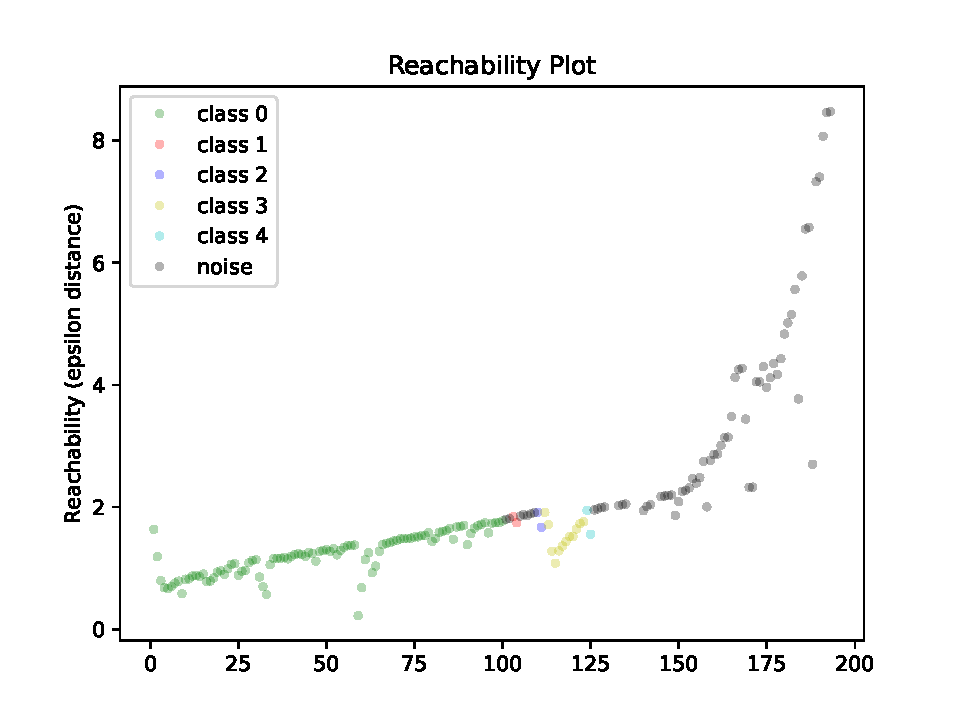
\includegraphics[width=5cm]{images/OPTICS/32x32/reachability_plot_32x32_pca_13dim.pdf} }}%
    \qquad
    \subfloat[\centering The reachability plot of the documents preprocessed according to \autoref{pt:eigendocs}.]{{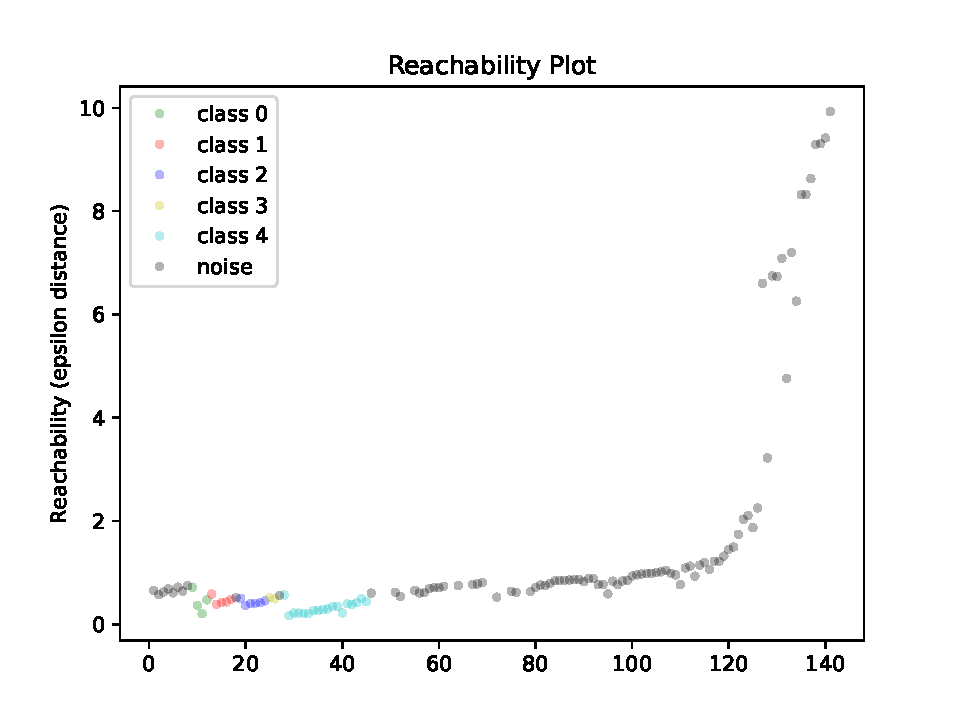
\includegraphics[width=5cm]{images/OPTICS/eigendocs/reachability_plot_13dim_eigendocs.pdf} }}%
    \caption{The plot was created using the \ac{optics} algorithm from the Python library scikit-learn.
    The plot shows the reachability distance of each document to its predecessor in the order list.
    The reachability distance is the minimum distance necessary to keep two consecutive objects in the same cluster.
    The plot shows that the documents are divided into a cluster and a noise region.}%
    \label{fig:reachability_plots}%
\end{figure}
